\subsection{Redes Neuronales Convolucionales}

\subsubsection{Introducción}

Sin duda alguna en la ultima década las redes neuronales convolucionales se popularizaron en gran medida. Todo comenzó con una nueva forma de computación inspirada en modelos biológicos, los cuales consisten en sistemas con un gran numero de procesos interconectados funcionando en paralelo los cuales procesan información y tienen la capacidad de aprender a través de la experiencia.\par
La detección de objetos en imágenes es una tarea de suma importancia a la hora de realizar un sistema de navegación autónomo, las redes neuronales vienen a resolver el problema.\par
Dentro de las las redes neuronales hay distintos tipos y una de ellas son las redes neuronales convolucionales (CNN) las cuales están inspiradas en las neuronas de la corteza visual primaria del cerebro. Estos tipos de redes neuronales pueden dotar a los robots de visión y es por eso que vienen a resolver el problema.\par
De esta forma esta sección de la tesis se enfocara en aportar un marco teórico de las redes neuronales convolucionales.\par

\subsubsection{El perceptrón}

En 1957 Frank Rosenblatt comenzó el desarrollo de una red neuronal a la que denomino ''El perceptrón'' fue tal su aporte que hoy en día se lo utiliza para reconocer patrones. Este modelo fue capaz de generalizar, es decir que luego un aprendizaje de ciertos patrones, y a pesar de sus limitaciones (era incapaz de resolver la OR exclusiva y en general incapaz de clasificar clases no separables linealmente) era capaz de reconocer patrones que jamas se le hayan presentado.
La entrada de la función de activación se calcula como la suma ponderada de todas las entradas del perceptrón más un valor de bias.\par

\begin{figure}[!h]
\centering
    \begin{tikzpicture}[scale=1.2]
    % Draw input nodes
    \foreach \h [count=\hi ] in {$i_2$,$i_1$,$i_0$}{%
          \node[input] (f\hi) at (0,\hi*1.25cm-1.5 cm) {\h};
        }
    % Dot dot dot ... x_n
    \node[below=0.62cm] (idots) at (f1) {\vdots};
    \node[input, below=0.62cm] (last_input) at (idots) {$i_n$};
    % Draw summation node
    \node[functions] (sum) at (4,0) {\Huge$\sum$};
    \node[above=1cm] at (sum) {$\sum_{k=0}^j w_ki_k + bias$};
    % Draw bias node
    \node[bias] (biass) at (4,-3) {$bias$};
    \draw[myarrow] (biass) -- (sum);
    % Draw edges from input nodes to summation node
    \foreach \h [count=\hi ] in {$w_2$,$w_1$,$w_0$}{%
          \path (f\hi) -- node[weights] (w\hi) {\h} (sum);
          \draw[myarrow] (f\hi) -- (w\hi);
          \draw[myarrow] (w\hi) -- (sum);}
    % Dot dot dot ... w_n
    \node[below=0.05cm] (wdots) at (w1) {\vdots};
    \node[weights, below=0.45cm] (last_weight) at (wdots) {$w_n$};
    % Add edges for last node and last weight etc
    \path[draw,myarrow] (last_input) -- (last_weight);
    \path[draw,myarrow] (last_weight) -- (sum);
    % Draw node for activation function
    \node[functions] (activation) at (7,0) {};
    % Place activation function in its node
    \begin{scope}[xshift=7cm,scale=1.25]
        \addaxes
        % flexible selection of activation function
        \relu
        % \stepfunc
    \end{scope}
    % Connect sum to relu
    \draw[myarrow] (sum) -- (activation);
    \draw[myarrow] (activation) -- ++(1,0);
    % Labels
    \node[above=1cm]  at (f3) {Entradas};
    \node[above=1cm] at (w3) {Pesos};
    \node[above=1cm] at (activation) {Función de activación};
    \end{tikzpicture} 
\captionof{figure}{El perceptrón}
\label{fig:elperceptron}
\end{figure}

\subsubsection{¿Que es una red neuronal?}

Una red neuronal es un grupo interconecto de distintos elementos procesadores simples que operan en paralelo, cuya función se determina a partir de distintas características de la red, su estructura, la fuerza o pesos en las conexiones y el procesamiento realizado en cada nodo.\par
Muchas veces se la define como un aproximador universal. El modelo conocido como perceptrón multicapa esta compuesto por ''k'' capas de neuronas que están interconectadas y cada salida de cada neurona es la suma ponderada de todas las salidas de las neuronas de la capa anterior mas un valor de bías (\autoref{fig:elperceptron}).

\begin{figure}[!h]
\centering
\begin{tikzpicture}[scale=1.5]
 
% Input Layer
\foreach \i in {1,...,\inputnum}
{
    \node[circle, 
        draw=black!90,
        very thick,
        minimum size = 10mm,
        fill=white!30] (Input-\i) at (-1.5,-\i*1.2) {};
}
\node[above=1cm] at (Input-1) {Capa de entrada}; % nombre de la capa
 
% Hidden Layer
\foreach \i in {1,...,\hiddennum}
{
    \node[circle, 
        draw=black!90,
        very thick,
        minimum size = 10mm,
        fill=white!50,
        yshift=(\hiddennum-\inputnum)*5 mm
    ] (Hidden-\i) at (1.5,-\i*1.2) {};
}
\node[above=2cm] at (Hidden-1) {Capa oculta}; % nombre de la capa
\node[above=1cm] at (Hidden-1) {$a_j = f(\sum_{i=1}^N w_{ij}x_i + b_j)$}; % nombre de la capa

% Output Layer
\foreach \i in {1,...,\outputnum}
{
    \node[circle, 
        draw=black!90,
        very thick,
        minimum size = 10mm,
        fill=white!50,
        yshift=(\outputnum-\inputnum)*5 mm
    ] (Output-\i) at (4.5,-\i*1.2) {};
}
\node[above=2cm] at (Output-1) {Capa de salida}; % nombre de la capa
\node[above=1cm] at (Output-1) {$y_{k} = g(\sum_{j=1}^M w_{jk}a_{jk} + b_k)$}; % nombre de la capa

% Connect neurons In-Hidden
\foreach \i in {1,...,\inputnum}
{
    \foreach \j in {1,...,\hiddennum}
    {
        \ifthenelse{ \i = 1 } 
        {\draw[->, shorten >=1pt,myarrow,black] (Input-\i) -- (Hidden-\j) node [pos=0.3,above] {$w_{\i\j}$};} 
        {\draw[->, shorten >=1pt, gray] (Input-\i) -- (Hidden-\j);}
    }
}
 
% Connect neurons Hidden-Out
\foreach \i in {1,...,\hiddennum}
{
    \foreach \j in {1,...,\outputnum}
    {
        %\draw[->, shorten >=1pt] (Hidden-\i) -- (Output-\j);
        \ifthenelse{ \j = 1 } 
        {\draw[->, shorten >=1pt,myarrow,black] (Hidden-\i) -- (Output-\j) node [pos=0.2,above] {$a_{\i}$};} 
        {\draw[->, shorten >=1pt, gray] (Hidden-\i) -- (Output-\j);}
    }
}
 
% Inputs
\foreach \i in {1,...,\inputnum}
{            
    \draw[<-, shorten <=1pt] (Input-\i) -- ++(-1,0) node[left]{$x_{\i}$};
}
 
% Outputs
\foreach \i in {1,...,\outputnum}
{            
    \draw[->, shorten <=1pt] (Output-\i) -- ++(1,0) node[right]{$y_{\i}$};
}
 
\end{tikzpicture} 
\captionof{figure}{Perceptrón multicapa}
\label{fig:elperceptronmulticapa}
\end{figure}

Debido a que la salida de una determinada neurona de la capa ''k'' se calcula utilizando todas las salidas de la neurona anterior se denomina capa de neuronas ''fully conected''.\par

\begin{itemize}
    \item Vector x: Entrada de la capa (conformado por las salidas de cada una de las neuronas de la capa anterior).
    \item n: Cantidad de neuronas de la capa anterior.
    \item Vector y: Vector de salidas.
    \item m: Cantidad de neuronas de la capa a calcular.
    \item Matriz w: Coeficientes de la capa ''fully connected''.
    \item Vector b: Bias de la capa ''fully connected''.
\end{itemize}

\[
   \begin{bmatrix} 
    w_{11} & \dots  & w_{1n} \\
    \vdots & \ddots & \vdots \\
    w_{m1} & \dots  & w_{mn} 
    \end{bmatrix}
    *
    \begin{bmatrix} 
    x_{1} \\
    \vdots \\
    x_{n} 
    \end{bmatrix}
    +
    \begin{bmatrix} 
    b_{1} \\
    \vdots \\
    b_{m} 
    \end{bmatrix}
    =
    \begin{bmatrix} 
    y_{1} \\
    \vdots \\
    y_{m} 
    \end{bmatrix}
    = 
    \begin{bmatrix} 
    a_{1} \\
    \vdots \\
    a_{m} 
    \end{bmatrix}
\]

\subsubsection{Capas convolucionales}

La principal diferencia de una red neuronal convolucional de cualquier otro red neuronal es que utiliza una operación llama ''convolución'' en algunas de sus capas en vez de utilizar la multiplicación de matrices. Esta operación recibe como entrada una imagen y luego le aplica un filtro (también llamado ''kernel'') y retorna otra imagen con las características de la imagen de entrada.\par
A continuación el proceso: \par

\begin{figure}[!h]
    \centering
    \begin{tikzpicture}

    % Simbolo de conv
    \begin{scope}[shift={(4,-0.3)},rotate=45, scale=0.5]
        \draw[-] (0,0,0) circle(1cm);
        \draw[-] (0,-1)--(0,1)--cycle;
        \draw[-] (-1,0)--(1,0)--cycle;
    \end{scope}
    
    % igual
    \begin{scope}[shift={(10.5,-0.5)},rotate=0, scale=0.35]
        \draw[-] (-1,1)--(1,1)--cycle;
        \draw[-] (-1,0)--(1,0)--cycle;
    \end{scope}
    
     % Matriz de entrada
    \begin{scope}[tdplot_main_coords,line join=miter,font=\sffamily, xshift=0, yshift=0cm]
        \pgfmathsetmacro{\xstretch}{1}
        \edef\Cols{white, white, white}
        \edef\LstCols{{"white", "white", "white"}}
        
        \foreach \Col [count=\X starting from 0,remember=\X as \LastX] in \Cols
        {  
            \foreach \XX in {1}
            {  
                \draw[thick,\Col] (\xstretch*\X+0.4*\XX-0.1,0,0) -- (\xstretch*\X+0.4*\XX,0,0);
                \begin{scope}[canvas is yz plane at x=\xstretch*\X+0.4*\XX]
                    \pgfmathtruncatemacro{\fullness}{120-20*\XX}
                    \draw[fill=\Col!\fullness] (-1,-1) rectangle (1,1);
                \end{scope}
            }
            %\node[anchor=west] at (\xstretch*\X,-2,-2){$x_\X$};
        }
        \node[anchor=west] at (\xstretch,-1.5,-1.5){$N_{iz}$};
        \node[anchor=west] at (\xstretch,1,-2.5){$N_{ix}$};
        \node[anchor=west] at (\xstretch,2.5,-1.5){$N_{iy}$};
        \node[anchor=west] at (\xstretch,-1,3){Matriz de entrada};
    \end{scope}
    % cuadraditos en la matriz de entrada
    \begin{scope}[tdplot_main_coords,line join=miter,font=\sffamily, xshift=-5, yshift=5, scale=0.2]
        \pgfmathsetmacro{\xstretch}{1}
        \edef\Cols{white, white, white}
        \edef\LstCols{{"white", "white", "white"}}
        
        \foreach \Col [count=\X starting from 0,remember=\X as \LastX] in \Cols
        {  
            \foreach \XX in {1}
            {  
                \draw[thick,\Col] (\xstretch*\X+0.4*\XX-0.1,0,0) -- (\xstretch*\X+0.4*\XX,0,0);
                \begin{scope}[canvas is yz plane at x=5*\xstretch*\X+0.4*\XX]
                    \pgfmathtruncatemacro{\fullness}{120-20*\XX}
                    \draw[fill=\Col!\fullness, draw=red] (-1,-1) rectangle (1,1);
                \end{scope}
            }
            %\node[anchor=west] at (\xstretch*\X,-2,-2){$x_\X$};
        }
    \end{scope}


    % Grupo de filtros
    \begin{scope}[tdplot_main_coords,line join=miter,font=\sffamily, xshift=5.5cm, yshift=0.2cm, scale=0.6]
        \pgfmathsetmacro{\xstretch}{1}
        \edef\Cols{red, green, blue}
        \edef\LstCols{{"red", "green", "blue"}}
        
        \foreach \Col [count=\X starting from 0,remember=\X as \LastX] in \Cols
        {  
            \foreach \XX in {1,2,3,4}
            {  
                %\draw[thick,\Col] (\xstretch*\X+0.4*\XX-0.1,0,0) -- (\xstretch*\X+0.4*\XX,0,0);
                \begin{scope}[canvas is yz plane at x=3.5*\xstretch*\X+0.4*\XX]
                    \pgfmathtruncatemacro{\fullness}{120-20*\XX}
                    \draw[fill=\Col!\fullness] (-1,-1) rectangle (1,1);
                \end{scope}
            }
            %\node[anchor=west] at (\xstretch*\X,-2,-2){$x_\X$};
        }
        \node[anchor=west] at (\xstretch,-1,4){Grupo de filtros};
        \node[anchor=west] at (5,0,-3.5){$N_{iz}$};
        \node[anchor=west] at (6,2,-4){$N_{wx}$};
        \node[anchor=west] at (7.5,2.5,-1){$N_{wy}$};
    \end{scope}
    
    % Matriz de salida
    \begin{scope}[tdplot_main_coords,line join=miter,font=\sffamily, xshift=350, yshift=0cm]
        \pgfmathsetmacro{\xstretch}{1}
        \edef\Cols{red, green, blue}
        \edef\LstCols{{"red", "green", "blue"}}
        
        \foreach \Col [count=\X starting from 0,remember=\X as \LastX] in \Cols
        {  
            \foreach \XX in {1}
            {  
                \draw[thick,\Col] (\xstretch*\X+0.4*\XX-0.1,0,0) -- (\xstretch*\X+0.4*\XX,0,0);
                \begin{scope}[canvas is yz plane at x=\xstretch*\X+0.4*\XX]
                    \pgfmathtruncatemacro{\fullness}{120-20*\XX}
                    \draw[fill=\Col!\fullness] (-1,-1) rectangle (1,1);
                \end{scope}
            }
            %\node[anchor=west] at (\xstretch*\X,-2,-2){$x_\X$};
        }
        \node[anchor=west] at (\xstretch,-1.5,-1.5){$N_{oz}$};
        \node[anchor=west] at (\xstretch,1,-2.5){$N_{ox}$};
        \node[anchor=west] at (\xstretch,2.5,-1.5){$N_{oy}$};
        \node[anchor=west] at (\xstretch,-1,3){Matriz de salida};
    \end{scope}
    
    
\end{tikzpicture}


  
  %\draw[thick,\Col] (\xstretch*\X+0.4*4,0,0) coordinate(front-\X) -- (\xstretch*\X+1+0.4*4,0,0) coordinate(back-\X);
%  \begin{scope}[canvas is xy plane at z=0]
%   \ifnum\X>0
%    \foreach \Z in {0,...,\LastX}
%    {\pgfmathsetmacro{\mycol}{\LstCols[\Z]}
%    \draw[thick,\mycol,overlay] (front-\Z) to[out=-90,in=-90,looseness=1.5] (back-\X);}
%   \fi
%  \end{scope}
%  \begin{scope}[canvas is yz plane at x=\xstretch*\X+1+0.4*4,transform shape]
%   \ifnum\X=4
%    \node[draw,fill=white] (BN-\X) at (0,0) {Transition layer};
%   \else
%    \node[draw,fill=white] (BN-\X) at (0,0) {BN--RelU--Conv};
%   \fi
%  \end{scope}
%  \pgfmathtruncatemacro{\NextX}{\X+1}
%  \ifnum\X<4
%   \node[anchor=south west] at (BN-\X.north east) {$H_\NextX$};
%   \pgfmathsetmacro{\NextCol}{\LstCols[\NextX]}
%  \else 
%   \pgfmathsetmacro{\NextCol}{"black"} 
%  \fi 
%  \draw[thick,\NextCol] (\xstretch*\X+1+0.4*4,0,0) -- ({\xstretch*(\X+1)+0.4*4},0,0); 
    \captionof{figure}{Operación de convolución}
    \label{fig:opconvolucion}
\end{figure}

\begin{itemize}
    \item $N_{iz}:$ cantidad de canales de la matriz de entrada a la capa. 
    \item $N_{ix}:$ ancho de la matriz de entrada. 
    \item $N_{iy}:$ largo de la matriz de entrada.
    \item $N_{wx}:$ ancho de cada filtro (del grupo de filtros) de la capa.
    \item $N_{wy}:$ largo de cada filtro (del grupo de filtros) de la capa.
    \item $N_{oz}:$ cantidad de filtros de la capa o bien los canales de la matriz de salida.
    \item $N_{ox}:$ ancho de la matriz de salida.
    \item $N_{oy}:$ largo de la matriz de salida.
\end{itemize}

Las salidas de una determinada capa convolucional se obtiene al desplazar $N_{of}$ filtros de dimensiones $ N_{wx} x N_{wy} x N_{iz}$ por las salidas de la capa anterior. En cada desplazamiento se realiza una suma ponderada de las salidas de la capa anterior por los pesos del filtro.\par

A continuación se presenta su algoritmo en pseudocódigo.\par



\begin{algorithm}[H]
\caption{Algoritmo de convolución}\label{alg:cap}
\begin{algorithmic}
    \For{$(c = 0; c < N_{oz} ; ++c)$} \Comment{Selector de filtro}
    \For{$(i = 0; i < N_{ix}; ++i)$} \Comment{Eje X de la matriz de entrada}
    \For{$(j = 0; j < N_{iy}; ++j)$} \Comment{Eje Y de la matriz de entrada}
        \For{$(v = 0; v < N_{iz}; ++v)$} \Comment{Canales de la matriz de entrada}
        \For{$(k = 0; k < N_{wx}; ++k)$} \Comment{Eje X del filtro}
        \For{$(l = 0; l < N_{wy}; ++l)$} \Comment{Eje Y del filtro}
            \State $o[j,i,c] += i[l,k,v,j,i] * w[l,k,v,c]$
        \EndFor
        \EndFor
        \EndFor
        
    \State $o[j,i,c] += b[c]$
    \EndFor  
    \EndFor   
    \EndFor

        
\end{algorithmic}
\end{algorithm}
 

\paragraph{Funciones de activación}\mbox{}\\

Normalmente utilizadas luego de una capa convolucional (o ''full connected'', según corresponda) y su función es la de agregar alinealidades al comportamiento de la red. Aplican un valor a cada valor de entrada (descripto mediante una función matemática). A continuación una explicación de las mas utilizadas.\par

\subparagraph{Sigmoide}\mbox{}\\

Una capa de activación Sigmoide transforma todos los valores de la entrada a una escala del (0,1) en donde los valores muy altos tienden a 1 y los valores muy bajos a 0.

\begin{figure}[!h]
\centering
\scalebox{.5}{\begin{tikzpicture}[declare function={sigma(\x)=1/(1+exp(-\x));
sigmap(\x)=sigma(\x)*(1-sigma(\x));}]
\begin{axis}[domain=-6:6]
[   xmin=-6,
    xmax=6,
    axis x line=bottom,
    ytick={0,.5,1},
    ymax=1,
    axis y line=middle,
    samples=100,
    domain=-6:6,
    legend style={at={(1,0.9)}}     ]
    \addplot[blue,mark=none]   (x,{sigma(x)});
    \addplot[red,dotted,mark=none]   (x,{sigmap(x)});
    %\legend{$\sigma(x)$,$\sigma'(x)$}
\end{axis}
\end{tikzpicture} }
\captionof{figure}{Función de activación: Sigmoide}
\label{fig:sigmoide}
\end{figure}

\subparagraph{ReLu}\mbox{}\\

Una capa de activación ReLu reemplaza todos los valores negativos recibidos a su entrada por ceros, su propósito es hacer el modulo alineal.

\begin{figure}[!h]
\centering
\scalebox{.5}{\begin{tikzpicture}
    \begin{axis}[domain=-3:5,]
        \addplot+[mark=none,red,domain=-3:0] {0};
        \addplot+[mark=none,red,domain=0:5] {x};
    \end{axis}
\end{tikzpicture} }
\captionof{figure}{Función de activación: ReLu}
\label{fig:relu}
\end{figure}

\paragraph{Método de submuestreo: capa de Pooling}\mbox{}\\

La capa de Pooling tiene como objetivo submuestrear la matriz de entrada reduciendo su tamaño. Una de sus principales ventajas es la de reducir el costo computacional de la red neuronal convolucional completa ya que reduce la cantidad de parámetros que esta tiene que aprender. A continuación una explicación de las mas utilizadas a la hora de construir una red neuronal convolucional. \par 

\subparagraph{Max Pooling}\mbox{}\\
\bigbreak

Max Pooling consiste en tomar una ''ventana'' de la matriz de entrada y efectuar una operación fija que retorne un escalar. En este caso retorna el valor máximo de la ventana y lo asigna como salida. A modo de ejemplo:\par

\begin{figure}[!h]
    \centering
    \begin{tikzpicture}
    \fill [red]    (0, 0)    rectangle (2, 2);
    \fill [yellow] (2, 0)    rectangle (4, 2);
    \fill [blue]   (2, 2)    rectangle (4, 4);
    \fill [green]  (0, 2)    rectangle (2, 4);

    \fill [red]    (9.5, 1)  rectangle (10.5, 2);
    \fill [yellow] (10.5, 1) rectangle (11.5, 2);
    \fill [blue]   (10.5, 2) rectangle (11.5, 3);
    \fill [green]  (9.5, 2)  rectangle (10.5, 3);

    \node at (0.5, 0.5) {7};
    \node at (1.5, 0.5) {9};
    \node at (2.5, 0.5) {3};
    \node at (3.5, 0.5) {5};
    %
    \node at (0.5, 1.5) {0};
    \node at (1.5, 1.5) {7};
    \node at (2.5, 1.5) {0};
    \node at (3.5, 1.5) {0};
    %
    \node at (0.5, 2.5) {2};
    \node at (1.5, 2.5) {0};
    \node at (2.5, 2.5) {9};
    \node at (3.5, 2.5) {3};
    %
    \node at (0.5, 3.5) {9};
    \node at (1.5, 3.5) {2};
    \node at (2.5, 3.5) {9};
    \node at (3.5, 3.5) {6};
    
    \node at (10, 1.5) {9};
    \node at (11, 1.5) {5};
    \node at (10, 2.5) {9};
    \node at (11, 2.5) {9};

    \draw[myarrow] (5, 2) -- (9,2);
    \node[font=\footnotesize\bfseries] at (6.5, 2.5) {$\mathbf{2\times 2}$ max pooling};
\end{tikzpicture}
 
    \captionof{figure}{Max Pooling}
    \label{fig:maxpooling}
\end{figure}

\subparagraph{Average Pooling}\mbox{}\\

Average Pooling consiste en tomar una ''ventana'' de la matriz de entrada y efectuar una operación fija que retorne un escalar. En este caso retorna el valor medio de la ventana y lo asigna como salida. A modo de ejemplo:\par

\begin{figure}[!h]
    \centering
    \begin{tikzpicture}
    \fill [red]    (0, 0)    rectangle (2, 2);
    \fill [yellow] (2, 0)    rectangle (4, 2);
    \fill [blue]   (2, 2)    rectangle (4, 4);
    \fill [green]  (0, 2)    rectangle (2, 4);

    \fill [red]    (9.5, 1)  rectangle (10.5, 2);
    \fill [yellow] (10.5, 1) rectangle (11.5, 2);
    \fill [blue]   (10.5, 2) rectangle (11.5, 3);
    \fill [green]  (9.5, 2)  rectangle (10.5, 3);

    \node at (0.5, 0.5) {12};
    \node at (1.5, 0.5) {12};
    \node at (2.5, 0.5) {45};
    \node at (3.5, 0.5) {6};
    %
    \node at (0.5, 1.5) {12};
    \node at (1.5, 1.5) {12};
    \node at (2.5, 1.5) {7};
    \node at (3.5, 1.5) {2};
    %
    \node at (0.5, 2.5) {0};
    \node at (1.5, 2.5) {100};
    \node at (2.5, 2.5) {70};
    \node at (3.5, 2.5) {38};
    %
    \node at (0.5, 3.5) {31};
    \node at (1.5, 3.5) {15};
    \node at (2.5, 3.5) {28};
    \node at (3.5, 3.5) {184};
    
    \node at (10, 1.5) {12};
    \node at (11, 1.5) {15};
    \node at (10, 2.5) {36};
    \node at (11, 2.5) {80};

    \draw[myarrow] (5, 2) -- (9,2);
    \node[font=\footnotesize\bfseries] at (6.5, 2.5) {$\mathbf{2\times 2}$ average pooling};
\end{tikzpicture}
 
    \captionof{figure}{Average Pooling}
    \label{fig:averagepooling}
\end{figure}

\paragraph{Capa de concatenación}\mbox{}\\

Esta capa es la encargada de tomar las entradas y concatenarlas a lo largo de una dimensión especifica, la única condición es que las entradas deben tener el mismo tamaño en todas las dimensiones excepto en la dimensión de concatenación.\par

\paragraph{Otras capas que suelen aparecer en una red neuronal convolucional}\mbox{}\\

Existen otras capas que suelen aparecer en algunas redes neuronales convolucionales como por ejemplo la capa de Dropout la cual consiste en desconectar un porcentaje de las neuronas en cada iteración del entrenamiento lo cual mejor la generalización de la red y ayuda a converger el entrenamiento.\par
La Normalización por lotes (mas conocida en ingles por ''Batch normalization'') que consiste en añadir un capa entre las neuronas y la función de activación para normalizar las activaciones de salida.\par
Existen algunas capas como la capa de convolución transpuesta (también conocida como capa de deconvolucion o capa de convolución fraccional) la cual se la utiliza para recuperar las dimensiones reducidas. Por ejemplo, luego de realizar una convolución con un step mayor que uno lo cual reduce el tamaño de la matriz de salida.\par


\subsubsection{Arquitectura de una red neuronal convolucional}

Una arquitectura de una red neuronal convolucional normalmente esta formada por una pila de capas distintas que transforman la matriz de entrada en una matriz de salida a través de una función diferenciable.\par
Algunas características importantes en las arquitecturas son: Los formatos de entrada/salida, la cantidad de capas de la red, parámetros de cada capa, la secuencia y forma de conexión de las capas entre si, y el algoritmo de entrenamiento. \par

Algunas redes y sus arquitecturas:

\begin{itemize}
    \item LeNet-5: 2 capas convolucionales y 3 ''fully connected''. Al rededor de 60.000 parámetros. Año 1998.
    \begin{center}
        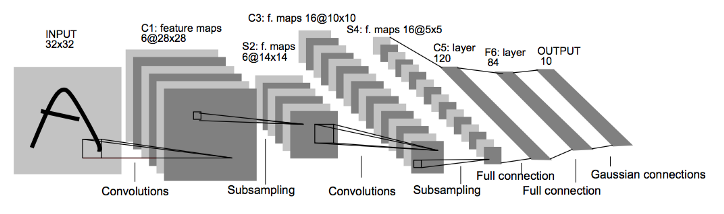
\includegraphics[scale=0.6]{Tesis/Capitulos/02_MARCO_TEORICO/img/LeNet5.png}
        \captionof{figure}{LeNet-5}
    \end{center}
    
    \item AlexNet: 8 capas, 3 ''fully connected'' y 5 convolucionales. Al rededor de 60 millones de parametros. Año 2012.
    
    \item VGG-16: 13 capas convolucionales y 3 ''fully connected''. Al rededor de 138 millones de parametros. Año 2014.
    
    \item ResNet-50: 50 capas, con modulos llamados ''ResNet'' (cada uno de 2 o 3 capas convolucionales). Al rededor de 26 millones de parametros. Año 2015.
    \begin{center}
        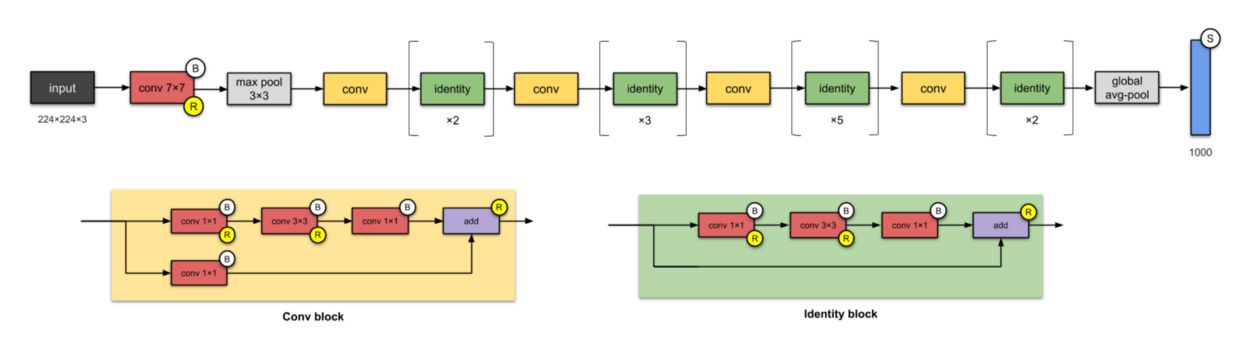
\includegraphics[scale=0.35]{Tesis/Capitulos/02_MARCO_TEORICO/img/ResNet50.png}
        \captionof{figure}{ResNet-50, de Raimi Karim, towardsdatascience}
    \end{center}
\end{itemize}

\subsubsection{Micro-arquitectura de una red neuronal convolucional}

La micro-arquitectura hace referencia a las capas individuales y/o módulos. A modo de ejemplo observemos el modulo ''ResNet'' de la red neuronal convolucionar ResNet-50.\par

\begin{figure}[H]
\hfill
\subfigure["Conv block" (Bloque de convolución)]{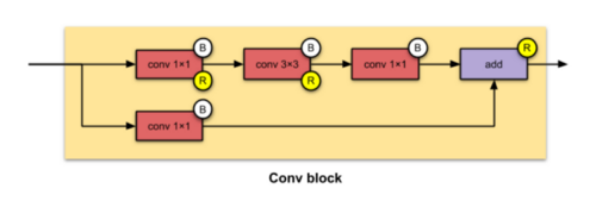
\includegraphics[width=5cm]{Tesis/Capitulos/02_MARCO_TEORICO/img/ResNetBlock1.png}}
\hfill
\subfigure[Identity block (Bloque de identidad)]{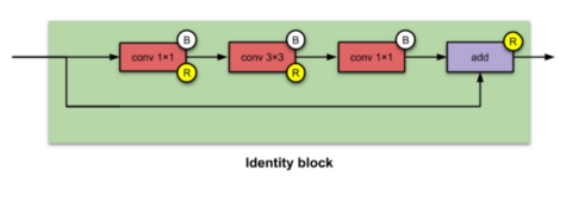
\includegraphics[width=5cm]{Tesis/Capitulos/02_MARCO_TEORICO/img/ResNetBlock2.png}}
\hfill
\caption{ResNet-50 modulo}
\end{figure}


\subsubsection{Entrenamiento de la red}

\paragraph{Introducción}\mbox{}\\

La fase de entrenamiento de la red neuronal convolucional consiste en, a partir de un set de imágenes de entrenamiento y sus respectivas etiquetas de los objetos a reconocer realizar iteraciones (también llamadas épocas) para ir determinando los pesos de cada uno de las neuronas en la red. Esta determinación se realiza a través del método de calculo conocido como ''Backpropagation''.\par
\bigbreak
Entonces en cada época, la etapa de entrenamiento se divide en dos etapas: Una fase directa (o hacia adelante) en donde una matriz de entrada pasa a través de toda la red neuronal. Se comparan las salidas obtenidas con las deseadas y se calcula el error para una de las salidas.\par
Y una fase inversa (o hacia atrás) donde los gradientes se pasan hacia atrás y los pesos se actualizan. Cada capa recibe un gradiente de perdida respecto a la salida y devuelve un gradiente de perdida respecto a la entrada. \par

Algo a tener en cuenta es que la fase de retroceso necesita datos que son almacenados durante la fase hacia adelante ya que se guardan datos de cada capas (entradas y valores intermedios) por lo que antes de realizar la propagación hacia atrás ''backpropagation'' es necesario una propagación hacia adelante ''forward propagation''. \par

\paragraph{Función de perdida}\mbox{}\\

Como mencione anteriormente finalizando la fase directa o de propagación hacia adelante se comparan las salidas obtenidas con las deseadas y se calcula el error para cada una de ellas. Esto se realiza a través de la Función de perdida $J_{(W)}$.\par
Es una tarea importante, en este proceso, la elección de la función de perdida que se va a minimizar. Ésta relaciona el valor esperado con los valores obtenido en la propagación hacia adelante.\par

\subparagraph{Entropía cruzada}\mbox{}\\

La entropía cruzada es una función de perdida típicamente utilizada para la clasificación de imágenes.\par

\begin{equation}
\tcboxmath[colback=white!25!white,colframe=black]
{ L = -ln(p_c) }  
\end{equation}

En donde ''c'' es la clase correcta y $p_c$ es la probabilidad predicha para la clase ''c''.\par

\paragraph{Desarrollo matemático}\mbox{}\\

Entonces, en la fase de la propagación hacia adelante, matemáticamente hablando se parte de una red en donde $a^{(l)}=f(z^{(l)})$ es la salida de la capa ''l'', tal que $z^{(l)}$ es el vector de pre-activación y se puede generalizar como $z^{(l)}=W^{(l)}*a^{(l-1)}$ siendo W los coeficientes de la capa y ''a'' la salida de la capa anterior y por ultimo $f()$, la función de activación de la capa l. \par
\bigbreak
Por otro lado, en la fase de propagación hacia atrás, matemáticamente hablando se utiliza un método de calculo de gradiente conocido como retropropagación y para poder utilizar este método es necesario encontrar las derivadas parciales de la función de perdida respecto a cada uno de los parámetros de la red $\frac{\partial J(W)}{\partial W^{l}_{ij}}$.\par

\begin{itemize}
    \item Se parte de Calcular el error y el delta de salida:
    \begin{enumerate}
        \item $e^{(L)} = d - a^{(L)}$ tal que ''L'' es la ultima capa, ''d'' el valor que debería dar a la salida y ''a'' el valor de la salida obtenido previamente en la propagación hacia adelante.
        \item $ \delta ^{(L)} = f'(z^{(L)}) \cdot e^{(L)}$ siendo $f'(z^{(L)}$ la derivada de la función de activación de la capa de salida.
    \end{enumerate}
    \item Para cada capa de la red neuronal se procede a calcular sus errores y deltas.
    \begin{enumerate}
        \item $e^{(L)} = W^{(l+1)^T} - \delta ^{(l+1)}$ tal que ''L'' es la ultima capa, ''d'' el valor que debería dar a la salida y ''a'' el valor de la salida obtenido previamente en la propagación hacia adelante.
        \item $ \delta ^{(L)} = f'(z^{(L)}) \cdot e^{(L)}$ siendo $f'(z^{(L)}$ la derivada de la función de activación de la capa de salida.
    \end{enumerate}
    \item Actualizamos las matrices de pesos.
    \begin{enumerate}
        \item $\Delta W^{(l)} = \lambda * (\delta^{(l)} \times a^{(l-1)} )$ tal que $\lambda$ se define como el factor de aprendizaje, y $a^{(l-1)}$ la salida de la neurona anterior.
        \item Actualización: $ W^{(l)} \leftarrow W^{(l)} + \Lambda W^{(l)} $
    \end{enumerate}
\end{itemize}

Este proceso se repite periódicamente (épocas) hasta alcanzar el entrenamiento deseado de la red.\par
